\chapter{Preconditioning}

Most recently, efforts have been directed at combining these three virtues of smoothed convergence curves, look-ahead to avoid breakdowns, and transposefree operation. So far, all three have not yet been combined fully satisfactorily in a single algorithm, but this research area is young.

\section{Preconditioners for $ Ax=b $} 
Given $ A\in \RR^{m\times m}, b\in \RR^{m} $, we want to solve 
\[
    Ax =b.
\]
For any nonsingular $ M\in \RR^{m\times m} $, the system 
\[
    M^{-1}  A x = M^{-1}  b
\]
has the same solution. However this system depends on the properties of $ M^{-1} A $ instead of just $ A $.  We call $ M $ the preconditioned. We don't need an explicit construction of the inverse $ M^{-1}  $, but the solution of systems of equations of the form 
\[
    My = c.
\]
The idea is that we find an $ M $ that we can solve $ My=c $ quickly, and $ M $ is very close to $ A $ which makes $ M^{-1} Ax = M^{-1} b$ easy. 

What does it mean for $M$ to be "close enough to $A ? "$ Answering this question is the matter that has occupied our attention throughout this part of the book. If the eigenvalues of $M^{-1} A$ are close to 1 and $\left\|M^{-1} A-I\right\|_2$ is small, then any of the iterations we have discussed can be expected to converge quickly. However, preconditioners that do not satisfy such a strong condition may also perform well. For example, the eigenvalues of $M^{-1} A$ could be clustered about a number other than 1 , and there might be some outlier eigenvalues far from the others.

For most problems involving iterations other than CGN, fortunately, a simple rule of thumb is adequate. A preconditioner $M$ is good if $M^{-1} A$ is not too far from normal and its eigenvalues are clustered.

\section{Left, Right, Hermitian Preconditioners} 
What we have described is a \textbf{left preconditioner}. Another idea is to transform $ Ax=b $ into $ AM^{-1} y=b $ with $ x=M^{-1} y $, in which case $ M $ is called a right preconditioner. 

If $ A $ is hermitian positive definite, then it is usal to preserve this property  in preconditioning. Suppose $ M $ is also PSD, with $ M = CC^*  $. Then the left preconditioner is equivalent to 
\[
    [C^{-1}  A C^{-*}] C^* x = C^{-1} b.
\]
This can be solve by CG. Besides, $ C^{-1}  A C^{-*} \sim M^{-1} A$. Hence, it's enough to examine the eigenvalues of $ M^{-1} A $. 

\section{Examples} 
Figure 40.1 presents an example of a preconditioned CG iteration for a symmetric positive definite matrix. The matrix $A$ isis the $1000 \times 1000$ symmetric matrix whose entries are all zero except for $a_{i j}=0.5+\sqrt{i}$ on the diagonal, $a_{i j}=1$ on the sub- and superdiagonals, and $a_{i j}=1$ on the 100 th sub- and superdiagonals, i.e., for $|i-j|=100$. The righthand side is $b=(1,1, \ldots, 1)^T$. As the figure shows, a straight CG iteration for this matrix converges slowly, achieving about five-digit residual reduction after forty iterations. Since the matrix is very sparse, this is an improvement over a direct method, but one would like to do better.

As it happens, we can do much better with a simple diagonal preconditioner. Take $M=\operatorname{diag}(A)$, the diagonal matrix with entries $m_{i i}=0.5+\sqrt{i}$. To preserve symmetry, set $C=\sqrt{M}$ and consider a new iteration. The figure shows that thirty steps of the iteration now give convergence to fifteen digits.

%────────────────────────────────────────
\begin{figure}[H]
    \centering
    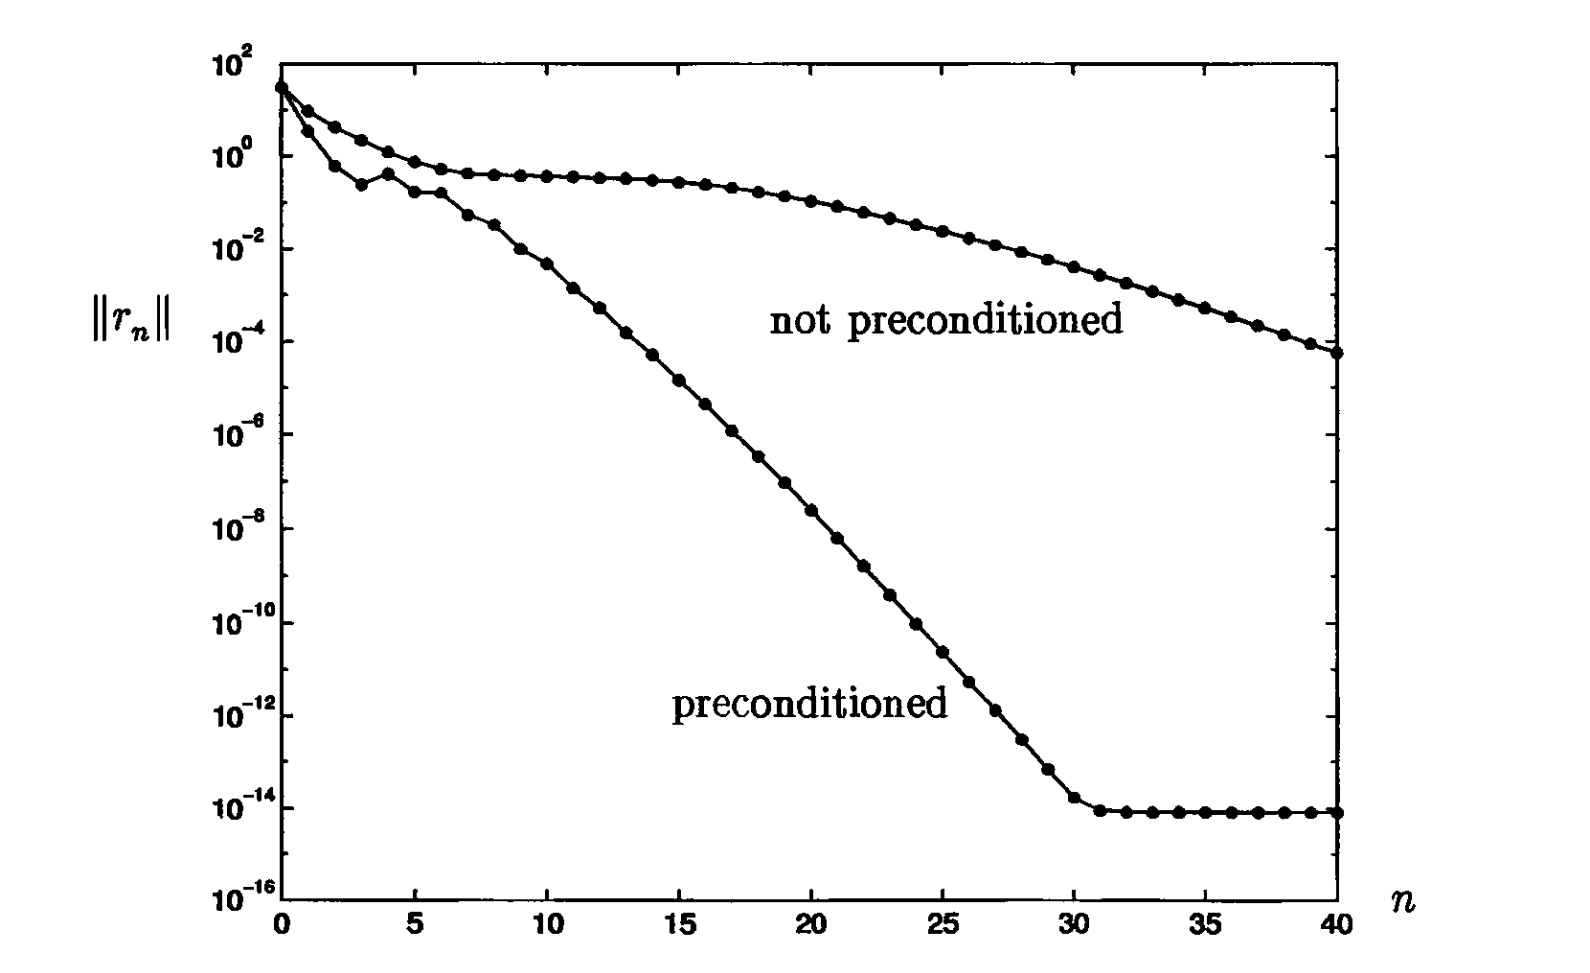
\includegraphics[width=0.8\textwidth]{figures/40-1.png}
    \caption{CG and preconditioned CG convergence curves for the $ 1000\times 1000 $ sparse matrix $ A $ described in the text. }
\end{figure}
%────────────────────────────────────────

\section{Survey of Preconditioners for $ Ax=b $} 
The preconditioners used in practice are sometimes as simple as this one, but they are often far more complicated. Rather than consider one or two examples in detail, we shall take the opposite course and survey at a high level the wide range of preconditioning ideas that have been found useful over the years. Details can be found in the references listed in the Notes.
\begin{itemize}
    \item \textbf{Diagonal Scaling or Jacobi.} Perhaps the most important preconditioner is the one just mentioned in the example: $M=\operatorname{diag}(A)$, provided that this matrix is nonsingular. For certain problems, this transformation alone is enough to make a slow iteration into a fast one. More generally, one may take $M=\operatorname{diag}(c)$ for a suitably chosen vector $c \in \mathbb{C}^m$. It is a hard mathematical problem to determine a vector $c$ such that $\kappa\left(M^{-1} A\right)$ is exactly minimized, but fortunately, nothing like the exact minimum is needed in practice, and in any case, as the rule of thumb above shows, there is more to preconditioning than minimizing the condition number.
    \item \textbf{Incomplete Cholesky or $L U$ factorization.} Another star preconditioner is the one that made the idea of preconditioning famous in the 1970s. Suppose $A$ is sparse, having just a few nonzeros per row. The difficulty with methods such as Gaussian elimination or Cholesky factorization is that these processes destroy zeros, so that if $A=R^* R$, for example, then the factor $R$ will usually not be very sparse. However, suppose a matrix $\tilde{R}$ is computed by Choleskylike formulas but allowed to have nonzeros only in positions where $A$ has nonzeros, and we define $M=\tilde{R}^* \tilde{R}$. This incomplete Cholesky preconditioner may be highly effective for some problems; the acronym ICCG for incomplete Cholesky conjugate gradients is used. Similar $I L U$ or incomplete $L U$ preconditioners are useful in nonsymmetric cases. Numerous variants of the idea of incomplete factorization have been proposed and developed extensively.
    \item \textbf{Coarse-grid approximation.} A discretization of a partial differential or integral equation on a fine grid may lead to a huge system of equations. The analogous discretization on a coarser grid, however, may lead to a small system that is easy to solve. If a method can be found to transfer solutions on the coarse grid to the fine grid and back again, e.g. by interpolation, then a powerful preconditioner may be obtained of the following schematic form:
    $$
    M=\langle\text { transfer to fine grid }\rangle \circ A_{\text {coarse }} \circ\langle\text { transfer to coarse grid }\rangle .
    $$
    Typically a preconditioner of this kind does a good job of handling the low-frequency components of the original problem, leaving the high frequencies to be treated by the Krylov subspace iteration. When this technique is iterated, resulting in a sequence of coarser and coarser grids, we obtain the idea of multigrid iteration.
    \item \textbf{Local approximation.} A coarse-grid approximation takes into account some of the larger-scale structure of a problem while ignoring some of the finer structure. A kind of a converse to this idea is relevant to problems $A x=b$ where $A$ represents coupling between elements both near and far from one another. The elements may be physical objects such as particles, or they may be numerical objects such as the panels introduced in a boundary element discretization. In any case, it may be worth considering the operator $M$ analogous to $A$ but with the longer-range interactions omitted-a short-range approximation to $A$. In the simplest cases of this kind, $M$ may consist simply of a few of the diagonals of $A$ near the main diagonal, making this a generalization of the idea of a diagonal preconditioner.
    \item \textbf{Block preconditioners and domain decomposition.} Throughout numerical linear algebra, most algorithms expressed in terms of the scalar entries of a matrix have analogues involving block matrices. An example is that a diagonal or Jacobi preconditioner may be generalized to block-diagonal or block-Jacobi form. This is another kind of local approximation, in that local effects within certain components are considered while connections to other components are ignored. In the past decade ideas of this kind have been widely generalized in the field of domain decomposition, in which solvers for certain subdomains of a problem are composed in flexible ways to form preconditioners for the global problem. These methods combine mathematical power with natural parallelizability.
    \item \textbf{Low-order discretization. }Often a differential or integral equation is discretized by a higher-order method such as a fourth-order finite difference formula or a spectral method, bringing a gain in accuracy but making the discretization stencils bigger and the matrix less sparse. A lower-order approximation of the same problem, with its sparser matrix, may be an effective preconditioner. Thus, for example, one commonly encounters finite difference and finite element preconditioners for spectral discretizations.

    \item \textbf{Constant-coefficient or symmetric approximation. }Special techniques, like fast Poisson solvers, are available for certain partial differential equations with constant coefficients. For a problem with variable coefficients, a constantcoefficient approximation implemented by a fast solver may make a good preconditioner. Analogously, if a differential equation is not self-adjoint but is close in some sense to a self-adjoint equation that can be solved more easily, then the latter may sometimes serve as a preconditioner.
    \item \textbf{Splitting of a multi-term operator.} Many applications involve combinations of physical effects, such as the diffusion and convection that combine to make up the Navier-Stokes equations of fluid mechanics. The linear algebra result may be a matrix problem $A x=b$ with $A=A_1+A_2$ (or with more than two terms, of course), often embedded in a nonlinear iteration. If $A_1$ or $A_2$ is easily invertible, it may serve as a good preconditioner.
    \item \textbf{Dimensional splitting or ADI.} Another kind of splitting takes advantage of the fact that an operator such as the Laplacian in two or three dimensions is composed of analogous operators in each of the dimensions separately. This idea may form the basis of a preconditioner, and in one form goes by the name of $A D I$ or alternating direction implicit methods.
    \item \textbf{One step of a classical iterative method.} In this book we have not discussed the "classical iterations" such as Jacobi, Gauss-Seidel, SOR, or SSOR, but one or more steps of these iterations-particularly Jacobi and SSOR-often serve excellently as preconditioners. This is also one of the key ideas behind multigrid methods.
    \item \textbf{Periodic or convolution approximation.} Throughout the mathematical sciences, boundary conditions are a source of analytical and computational difficulty. If only there were no boundary conditions, so that the problem were posed on a periodic domain! This idea can sometimes be the basis of a good preconditioner. In the simplest linear algebra context, it becomes the idea of preconditioning a problem involving a Toeplitz matrix $A$ (i.e., $a_{i, j}=a_{i-j}$ ) by a related circulant matrix $M\left(m_{i, j}=m_{(i-j)(\bmod m)}\right)$, which can be inverted in $O(m \log m)$ operations by a fast Fourier transform. This is a particularly well studied example in which $M^{-1} A$ may be far from the identity in norm but have highly clustered eigenvalues.
    \item \textbf{Unstable direct method.} Certain numerical methods, such as Gaussian elimination without pivoting, deliver inaccurate answers because of instability. If the unstable method is fast, however, why not use it as a preconditioner? This is the "fly by wire" approach to numerical computation: solve the problem carelessly but quickly, and embed that solution in a robust control system. It is a powerful idea.
    \item \textbf{Polynomial preconditioners.} Finally, we mention a technique that is different from the others in that it is essentially $A^{-1}$ rather than $A$ itself that is approximated by the preconditioner. A polynomial preconditioner is a matrix polynomial $M^{-1}=p(A)$ with the property that $p(A) A$ has better properties for iteration than $A$ itself. For example, $p(A)$ might be obtained from the first few terms of the Neumann series $A^{-1}=I+(I-A)+(I-A)^2+\cdots$, or from some other expression, often motivated by approximation theory in the complex plane. Implementation is easy, based on the same "black box" used for the Krylov subspace iteration itself, and the coefficients of the preconditioner may sometimes be determined adaptively.
\end{itemize} 
\section{Preconditioners for Eigenvalue Problems} 
Though the idea has been developed more recently and is not yet as famous, preconditioners can be effective for eigenvalue problems as well as systems of equations. Some of the best-known techniques in this area are polynomial acceleration, analogous to the polynomial preconditioning just described for systems of equations, shift-and-invert Arnoldi or the related rational Krylov iteration, which employ rational functions of $A$ instead of polynomials, and the Davidson and Jacobi-Davidson methods, based on a kind of diagonal preconditioner. For example, shift-and-invert and rational Krylov methods are based on the fact that if $r(z)$ is a rational function and $\left\{\lambda_j\right\}$ are the eigenvalues of $A$, then the eigenvalues of $r(A)$ are $\left\{r\left(\lambda_j\right)\right\}$. If $r(A)$ can be computed with reasonable speed and its eigenvalues are better distributed for iteration than those of $A$, this may be a route to fast calculation of eigenvalues.
\section{A Closing Note} 
In ending this book with the subject of preconditioners, we find ourselves at the philosophical center of the scientific computing of the future. The traditional view of computer scientists is that a computational problem is finite: after a short or long calculation, one obtains the solution exactly. Over the years, however, this view has come to be appropriate to fewer and fewer problems. The best methods for large-scale computational problems are usually approximate ones, methods that obtain a satisfactorily accurate solution in a short time rather than an exact one in a much longer or infinite time. $\mathrm{Nu}-$ merical analysis is indeed a branch of analysis, primarily, not algebra-even when the problems to be solved are from linear algebra. Further speculations on this phenomenon are presented in the Appendix.

Nothing will be more central to computational science in the next century than the art of transforming a problem that appears intractable into another whose solution can be approximated rapidly. For Krylov subspace matrix iterations, this is preconditioning. For the great range of computational problems, both continuous and discrete, we can only guess where this idea will take us.
 